\documentclass[11pt,a4paper]{article}
\usepackage[margin=2.5cm]{geometry}
\usepackage[utf8]{inputenc}
\usepackage[T1]{fontenc}
\usepackage{hyperref}
\renewcommand{\familydefault}{\sfdefault}
\usepackage{helvet}
\pagestyle{empty}
\usepackage[kerning=true]{microtype}
\usepackage{parskip}
\usepackage{sansmath}
\usepackage[font={small, bf}]{caption}
\usepackage[font={small}]{subcaption}
\usepackage{graphicx}
\usepackage{multicol}
\setlength{\abovecaptionskip}{0pt}
\setlength{\floatsep}{10pt}
\setlength{\textfloatsep}{0pt}
\setlength{\intextsep}{0pt}
\setlength{\belowcaptionskip}{0pt}
\setlength{\parindent}{5ex}
\setlength{\parskip}{0pt}
% Feel free to use additional packages for glosses, figures, whatnot.

% The next bit is for reserving sufficient space for authors,
% affiliations, and e-mail address.  No need to change for initial
% anonymous version.  For the final version, replace the
% \toggletrue{anonymous} with \togglefalse{anonymous} to de-anonymize.
\usepackage{etoolbox}
\newtoggle{anonymous}
\toggletrue{anonymous}

\renewcommand{\title}[1]{\textbf{#1}\\}
\newcommand{\authors}[1]{\iftoggle{anonymous}{\phantom{#1}}{#1}\\}
\newcommand{\email}[1]{\iftoggle{anonymous}{\phantom{#1}}{#1}}

\begin{document}

% First page:

% Insert title, authors, affiliations, and e-mail address in the next three lines:

\title{TODO TITLE}
\authors{Veronica Boyce, Ilaria Chen, Bobby Sparks, Malia Perez, Michael C. Frank} 
\email{vboyce@stanford.edu;  Stanford University}
\newline
%

% Intro
%TODO citations


\textbf{Methods:} 

% Results

\textbf{Results:} 

\textbf{Conclusion:} 

\newpage

\begin{figure}

	\caption{Schematic of methods}
\end{figure}


	\begin{figure}
		\begin{minipage}{.5\textwidth}
			\captionof{figure}{Results}
			{	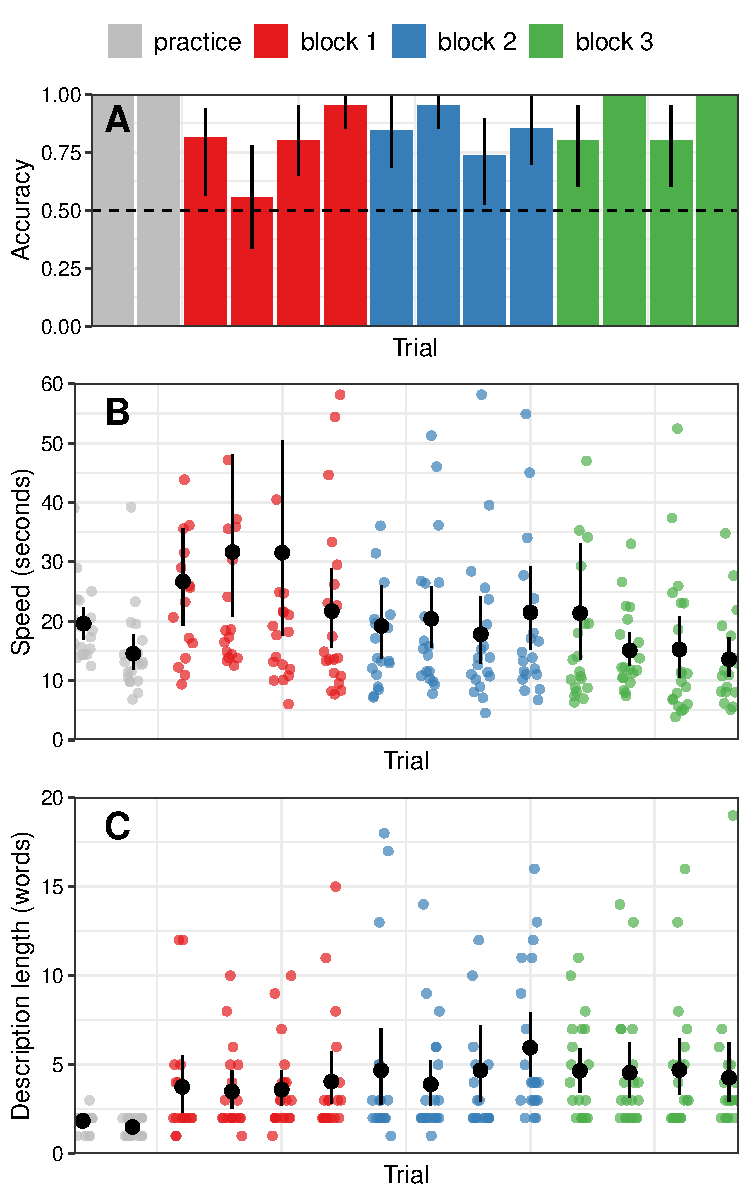
\includegraphics[width=\textwidth]{plot1.pdf}} 
			\begin{small}
				FOOBAR
				
			\end{small}
			
		\end{minipage}
		~~~
		\begin{minipage}{.5\textwidth}	
		\captionof{figure}{Similarity Results}
		{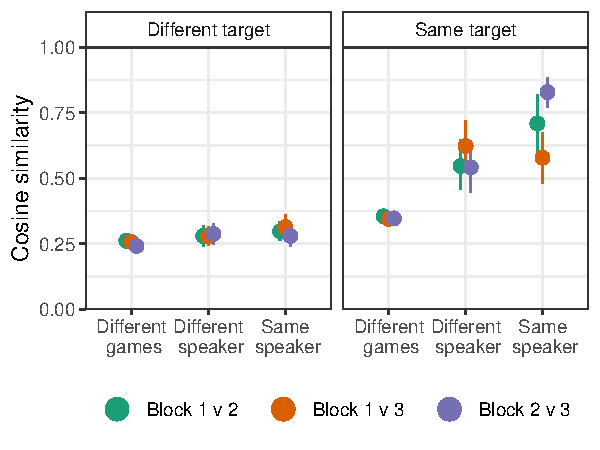
\includegraphics[width=\textwidth]{sims.pdf}} 
		\begin{small}
		Descriptions given by children were compared using sentence embeddings. Descriptions were most similar when provided by the same child for the same image. However, children described images more similarly to their partners than to children in other games.  
		\end{small}
		\end{minipage}
	\end{figure}



\begin{figure}\textbf{References:}

\end{figure}
\end{document}